\chapter{JVM Instr Set \& JIT}
\section{Instruction Set}
\section*{26 - Settembre}


Let's consider the instructions \textbf{format}.
Each instr may have different \textit{"forms"} supporting different kinds of operands.
For example there are different forms of \lst{iload} (i.e. push).

Runtime memory contains
- Local variable array (frame)
– Operand stack (frame)
– Object fields (heap)
– Static fields (method area)

Note that Java instructions are explicitly typed through \textbf{opCodes}, e.g. \lst{dload},\lst{iload},\lst{fload}.\\
\textbf{opCodes} are bytes, allowing only for 256 distinct ones;
hence it is impossible to have for each instruction on opCode per type.
The JVM specification indicates a selection of which types to support for each op instruction, and not supported types have to be converted; resulting in the Instruction Set Architecture to present non-orthogonality.\\
Types like \lst{byte}, \lst{char} and \lst{short} are usually converted to \lst{int} when performing computations.

\section*{27 - Settembre}

\subsection{Invoking methods}
\lst{invokevirtual} causes the allocation of a new frame, pops the arguments from the stack into the local variables of the caller (putting this in 0),
and passes the control to it by changing the \lst{pc}.
\begin{itemize}
    \item A resolution of the symbolic link is performed
    \item \lst{ireturn} pushes the top of the current stack to the stack of the caller, and passes the control to it. Similarly for \lst{dreturn}, \lst{freturn} ...
    \item \lst{return} just passes the control to the caller
\end{itemize}

There are 4 others kinds of method invocation:
\begin{itemize}
    \item \lst{invokestatic}: call methods with \lst{static} modifier; \textit{this} is not passed
    \item \lst{invokespecial}: call constructors, \lst{private} methods or \textit{superclass} methods; \textit{this} is always passed 
    \item \lst{invokeinterface}: identical to \lst{invokevirtual}, but used when the method is declared in an interface, thus a different lookup is required
    \item \lst{invokedynamic}: introduced in Java 7 to support dynamic typing\footnote{lambda functions related?}
\end{itemize}

(...)

\section{JIT}
\textit{AOT} \textbf{Ahead of Time} \textit{Compilation} leads to better performance in general, exploiting hardware features and variables allocation without runtime lookup;
While \textbf{Interpretation} facilitates interactive debugging and testing: it allows command-line invocation.

\textbf{JIT} aims to get the advantages of both.

\textit{JIT} differs from \textit{AOT} since it runs in the same process of the application and competes with the app for resources,
thus compilation time for JIT is more relevant than for an AOT Compiler.
Besides, a JIT compiler doesn't verify classes at compile time, it is a task performed by the JVM at load time. 
JIT can exploit new optimization possibilities, e.g. \textit{deoptimization} and \textit{speculation}.
A JIT takes bytecode as input and outputs machine code that the CPU executes directly.\\
Wrapping up:
\begin{itemize}
    \item Code starts executing interpreted with no delay
    \item Methods that are found commonly executed (\textit{hot}) are JIT compiled
    \item Once compiled code is available, the execution switches to it.
\end{itemize}

To identify \textit{hot} methods, there is a \textbf{threshold} on two \textit{per-method} counters:
\begin{enumerate}
    \item Times the method is invoked
    \item Times a brach back to the start of a loop is taken in the method
\end{enumerate}

A tradeoff between
"fast-to-start-but-slow-to-execute" interpreter vs "slow-to-
start-but-fast-to-execute" compiled code
is managed by a multi tier system.

(...)

\subsection{Deoptimization and Speculation}
Usually method executions pass in three phases:
\nl

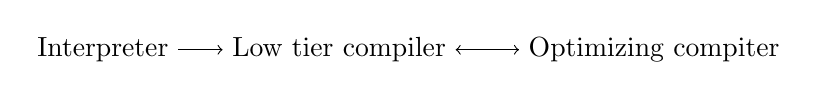
\begin{tikzpicture}
    \node[shape=rectangle,draw=white] (A) at (0,0) {Interpreter};
    \node[shape=rectangle,draw=white] (B) at (3,0) {Low tier compiler};
    \node[shape=rectangle,draw=white] (C) at (7,0) {Optimizing compiter};
    \path [->] (A) edge node[left] {} (B);
    \path [->] (B) edge node[left] {} (C);
    \path [->] (C) edge node[left] {} (B);    
\end{tikzpicture}

But sometimes \textbf{deoptimization} can happen, i.e. :
\nl

\begin{tikzpicture}[>=stealth',shorten >=1pt,auto,node distance=2.8cm]
    \node[shape=rectangle,draw=white] (A) at (0,0) {Interpreter};
    \node[shape=rectangle,draw=white] (B) at (3,0) {Low tier compiler};
    \node[shape=rectangle,draw=white] (C) at (7,0) {Optimizing compiter};

    \path [->] (A) edge node[left] {} (B);
    \path [->] (B) edge node[left] {} (C);
    \path [->] (C) edge [bend left] node {} (B);
    \path [->] (C) edge [bend left] node {} (A);
\end{tikzpicture}